\documentclass{article}

\usepackage{tikz}
\usetikzlibrary{arrows}
\usetikzlibrary{automata}
\usetikzlibrary{calc}
\usetikzlibrary{fit}
\usetikzlibrary{matrix}
\usetikzlibrary{positioning}

\begin{document}

\title{How Fragments Become an NFA:\\ Or, How Sausage is Made}
\maketitle

\begin{figure}
\centering
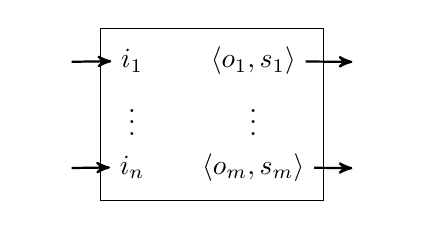
\begin{tikzpicture}

  \matrix [matrix of math nodes,column sep=0.5cm] {
    |(to_i_1)| \phantom{x} & |(i_1)| i_1 & |(o_1)| \langle o_1, s_1 \rangle & |(from_o_1)| \phantom{x} \\
    & \vdots & \vdots & \\
    |(to_i_n)| \phantom{x} & |(i_n)| i_n & |(o_m)| \langle o_m, s_m \rangle & |(from_o_m)| \phantom{x} \\
  };

  \node [draw,rectangle,fit=(i_1) (i_n) (o_1) (o_m)] {};

  \path [draw,thick,->,>=stealth',overlay]
    (to_i_1) edge (i_1)
    (to_i_n) edge (i_n)
    (o_1)    edge (from_o_1)
    (o_m)    edge (from_o_m);

\end{tikzpicture}
\caption{A fragment}
\end{figure}

\begin{figure}
\centering
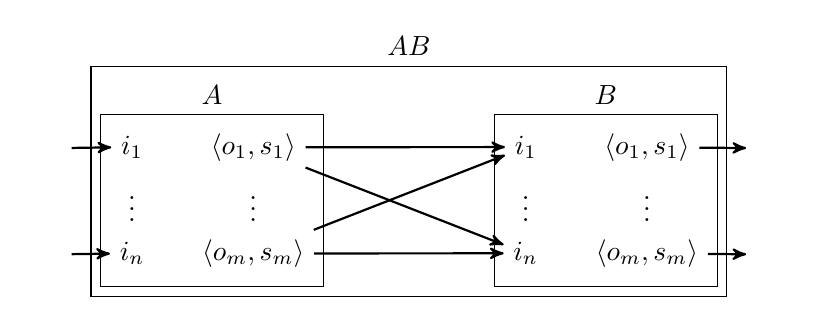
\begin{tikzpicture}

  \matrix [matrix of math nodes,column sep=0.5cm] at (-2.5,0) {
    |(Ato_i_1)| \phantom{x} & |(Ai_1)| i_1 & |(Ao_1)| \langle o_1, s_1 \rangle & |(Afrom_o_1)| \phantom{x} \\
    & \vdots & \vdots & \\
    |(Ato_i_n)| \phantom{x} & |(Ai_n)| i_n & |(Ao_m)| \langle o_m, s_m \rangle & |(Afrom_o_m)| \phantom{x} \\
  };

  \node [draw,rectangle,fit=(Ai_1) (Ai_n) (Ao_1) (Ao_m),label={[name=Alab]above:$A$}] (A) {};

  \path [draw,thick,->,>=stealth',overlay]
    (Ato_i_1) edge (Ai_1)
    (Ato_i_n) edge (Ai_n);

  \matrix [matrix of math nodes,column sep=0.5cm] at (2.5,0) {
    |(Bto_i_1)| \phantom{x} & |(Bi_1)| i_1 & |(Bo_1)| \langle o_1, s_1 \rangle & |(Bfrom_o_1)| \phantom{x} \\
    & \vdots & \vdots & \\
    |(Bto_i_n)| \phantom{x} & |(Bi_n)| i_n & |(Bo_m)| \langle o_m, s_m \rangle & |(Bfrom_o_m)| \phantom{x} \\
  };

  \node [draw,rectangle,fit=(Bi_1) (Bi_n) (Bo_1) (Bo_m),label={[name=Blab]above:$B$}] (B) {};

  \path [draw,thick,->,>=stealth',overlay]
    (Bo_1) edge (Bfrom_o_1)
    (Bo_m) edge (Bfrom_o_m);

  \path [draw,thick,->,>=stealth']
    (Ao_1) edge (Bi_1)
    (Ao_1) edge (Bi_n)
    (Ao_m) edge (Bi_1)
    (Ao_m) edge (Bi_n);

  \node [draw,rectangle,fit=(A) (Alab) (B) (Blab),label=above:$AB$] (AB) {};

\end{tikzpicture}
\caption{Concatenation: $A.k = B.k = \emptyset$}
\end{figure}

\begin{figure}
\centering
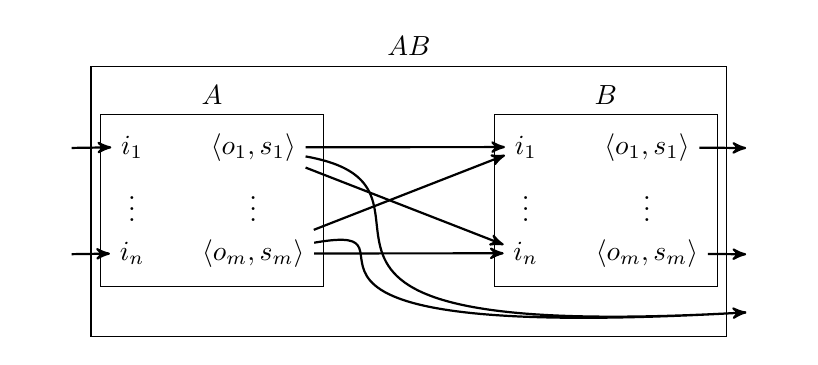
\begin{tikzpicture}

  \matrix [matrix of math nodes,column sep=0.5cm,anchor=north] at (-2.5,0) {
    |(Ato_i_1)| \phantom{x} & |(Ai_1)| i_1 & |(Ao_1)| \langle o_1, s_1 \rangle & |(Afrom_o_1)| \phantom{x} \\
    & \vdots & \vdots & \\
    |(Ato_i_n)| \phantom{x} & |(Ai_n)| i_n & |(Ao_m)| \langle o_m, s_m \rangle & |(Afrom_o_m)| \phantom{x} \\
  };

  \node [draw,rectangle,fit=(Ai_1) (Ai_n) (Ao_1) (Ao_m),label={[name=Alab]above:$A$}] (A) {};

  \path [draw,thick,->,>=stealth',overlay]
    (Ato_i_1) edge (Ai_1)
    (Ato_i_n) edge (Ai_n);

  \matrix [matrix of math nodes,column sep=0.5cm,anchor=north] at (2.5,0) {
    |(Bto_i_1)| \phantom{x} & |(Bi_1)| i_1 & |(Bo_1)| \langle o_1, s_1 \rangle & |(Bfrom_o_1)| \phantom{x} \\
    & \vdots & \vdots & \\
    |(Bto_i_n)| \phantom{x} & |(Bi_n)| i_n & |(Bo_m)| \langle o_m, s_m \rangle & |(Bfrom_o_m)| \phantom{x} \\[0.25cm]
    && |(B_skip)| & |(Bfrom_skip)| \phantom{x} \\
  };

  \node [draw,rectangle,fit=(Bi_1) (Bi_n) (Bo_1) (Bo_m),label={[name=Blab]above:$B$}] (B) {};

  \path [draw,thick,->,>=stealth',overlay]
    (Bo_1) edge (Bfrom_o_1)
    (Bo_m) edge (Bfrom_o_m);

  \path [draw,thick,->,>=stealth']
    (Ao_1) edge (Bi_1)
    (Ao_1) edge (Bi_n)
    (Ao_m) edge (Bi_1)
    (Ao_m) edge (Bi_n);

  \path [draw,thick,->,>=stealth',overlay]
    (Ao_1) .. controls +(-10:3cm) and +($(Bfrom_skip) + (170:12cm)$) .. (Bfrom_skip)
    (Ao_m) .. controls +(10:2.5cm) and +($(Bfrom_skip) + (170:12cm)$) .. (Bfrom_skip);


  \node [draw,rectangle,fit=(A) (Alab) (B) (Blab) (B_skip),label=above:$AB$] (AB) {};

\end{tikzpicture}
\caption{Concatenation: $A.k = \emptyset, B.k \ne \emptyset$}
\end{figure}

\begin{figure}
\centering
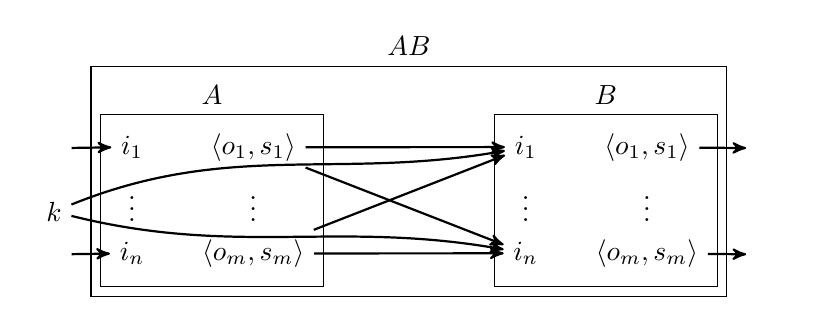
\begin{tikzpicture}

  \matrix [matrix of math nodes,column sep=0.5cm] at (-2.5,0) {
    |(Ato_i_1)| \phantom{x} & |(Ai_1)| i_1 & |(Ao_1)| \langle o_1, s_1 \rangle & |(Afrom_o_1)| \phantom{x} \\
    |(A_skip)| k & \vdots & \vdots & \\
    |(Ato_i_n)| \phantom{x} & |(Ai_n)| i_n & |(Ao_m)| \langle o_m, s_m \rangle & |(Afrom_o_m)| \phantom{x} \\
  };

  \node [draw,rectangle,fit=(Ai_1) (Ai_n) (Ao_1) (Ao_m),label={[name=Alab]above:$A$}] (A) {};

  \path [draw,thick,->,>=stealth',overlay]
    (Ato_i_1) edge (Ai_1)
    (Ato_i_n) edge (Ai_n);

  \matrix [matrix of math nodes,column sep=0.5cm] at (2.5,0) {
    |(Bto_i_1)| \phantom{x} & |(Bi_1)| i_1 & |(Bo_1)| \langle o_1, s_1 \rangle & |(Bfrom_o_1)| \phantom{x} \\
    & \vdots & \vdots & \\
    |(Bto_i_n)| \phantom{x} & |(Bi_n)| i_n & |(Bo_m)| \langle o_m, s_m \rangle & |(Bfrom_o_m)| \phantom{x} \\
  };

  \node [draw,rectangle,fit=(Bi_1) (Bi_n) (Bo_1) (Bo_m),label={[name=Blab]above:$B$}] (B) {};

  \path [draw,thick,->,>=stealth',overlay]
    (Bo_1) edge (Bfrom_o_1)
    (Bo_m) edge (Bfrom_o_m);

  \path [draw,thick,->,>=stealth']
    (Ao_1) edge (Bi_1)
    (Ao_1) edge (Bi_n)
    (Ao_m) edge (Bi_1)
    (Ao_m) edge (Bi_n);

  \node [draw,rectangle,fit=(A) (Alab) (B) (Blab),label=above:$AB$] (AB) {};

  \path [draw,thick,->,>=stealth',overlay]
    (A_skip) edge [out=22,in=190] (Bi_1)
    (A_skip) edge [out=-14,in=170] (Bi_n);

\end{tikzpicture}
\caption{Concatenation: $A.k \ne \emptyset, B.k = \emptyset$}
\end{figure}

\begin{figure}
\centering
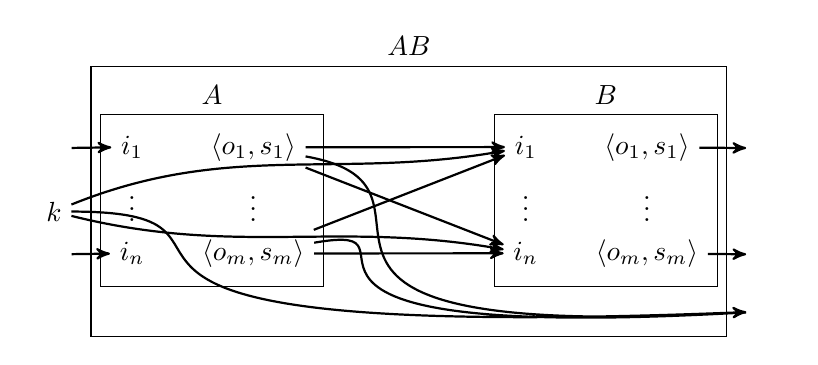
\begin{tikzpicture}

  \matrix [matrix of math nodes,column sep=0.5cm,anchor=north] at (-2.5,0) {
    |(Ato_i_1)| \phantom{x} & |(Ai_1)| i_1 & |(Ao_1)| \langle o_1, s_1 \rangle & |(Afrom_o_1)| \phantom{x} \\
    |(A_skip)| k & \vdots & \vdots & \\
    |(Ato_i_n)| \phantom{x} & |(Ai_n)| i_n & |(Ao_m)| \langle o_m, s_m \rangle & |(Afrom_o_m)| \phantom{x} \\
  };

  \node [draw,rectangle,fit=(Ai_1) (Ai_n) (Ao_1) (Ao_m),label={[name=Alab]above:$A$}] (A) {};

  \path [draw,thick,->,>=stealth',overlay]
    (Ato_i_1) edge (Ai_1)
    (Ato_i_n) edge (Ai_n);

  \matrix [matrix of math nodes,column sep=0.5cm,anchor=north] at (2.5,0) {
    |(Bto_i_1)| \phantom{x} & |(Bi_1)| i_1 & |(Bo_1)| \langle o_1, s_1 \rangle & |(Bfrom_o_1)| \phantom{x} \\
    & \vdots & \vdots & \\
    |(Bto_i_n)| \phantom{x} & |(Bi_n)| i_n & |(Bo_m)| \langle o_m, s_m \rangle & |(Bfrom_o_m)| \phantom{x} \\[0.25cm]
    && |(B_skip)| & |(Bfrom_skip)| \phantom{x} \\
  };

  \node [draw,rectangle,fit=(Bi_1) (Bi_n) (Bo_1) (Bo_m),label={[name=Blab]above:$B$}] (B) {};

  \path [draw,thick,->,>=stealth',overlay]
    (Bo_1) edge (Bfrom_o_1)
    (Bo_m) edge (Bfrom_o_m);

  \path [draw,thick,->,>=stealth']
    (Ao_1) edge (Bi_1)
    (Ao_1) edge (Bi_n)
    (Ao_m) edge (Bi_1)
    (Ao_m) edge (Bi_n);

  \node [draw,rectangle,fit=(A) (Alab) (B) (Blab) (B_skip),label=above:$AB$] (AB) {};

  \path [draw,thick,->,>=stealth',overlay]
    (A_skip) edge [out=22,in=190] (Bi_1)
    (A_skip) edge [out=-14,in=170] (Bi_n);

  \path [draw,thick,->,>=stealth',overlay]
    (Ao_1) .. controls +(-10:3cm) and +($(Bfrom_skip) + (170:12cm)$) .. (Bfrom_skip)
    (Ao_m) .. controls +(10:2.5cm) and +($(Bfrom_skip) + (170:12cm)$) .. (Bfrom_skip)
    (A_skip) .. controls +(0:3.25cm) and +($(Bfrom_skip) + (172:15cm)$) .. (Bfrom_skip);

\end{tikzpicture}
\caption{Concatenation: $A.k \ne \emptyset, B.k \ne \emptyset$}
\end{figure}


\end{document}
